\documentclass[]{article}
\usepackage{lmodern}
\usepackage{amssymb,amsmath}
\usepackage{ifxetex,ifluatex}
\usepackage{fixltx2e} % provides \textsubscript
\ifnum 0\ifxetex 1\fi\ifluatex 1\fi=0 % if pdftex
  \usepackage[T1]{fontenc}
  \usepackage[utf8]{inputenc}
\else % if luatex or xelatex
  \ifxetex
    \usepackage{mathspec}
  \else
    \usepackage{fontspec}
  \fi
  \defaultfontfeatures{Ligatures=TeX,Scale=MatchLowercase}
\fi
% use upquote if available, for straight quotes in verbatim environments
\IfFileExists{upquote.sty}{\usepackage{upquote}}{}
% use microtype if available
\IfFileExists{microtype.sty}{%
\usepackage{microtype}
\UseMicrotypeSet[protrusion]{basicmath} % disable protrusion for tt fonts
}{}
\usepackage[margin=1in]{geometry}
\usepackage{hyperref}
\hypersetup{unicode=true,
            pdftitle={A Dynamic Intrafamily Model of Child Behavior Problems and Birth Timing},
            pdfauthor={Charles C. Lanfear; Ross L. Matsueda},
            pdfkeywords={keyword 1; keyword 2; keyword 3},
            pdfborder={0 0 0},
            breaklinks=true}
\urlstyle{same}  % don't use monospace font for urls
\usepackage{longtable,booktabs}
\usepackage{graphicx,grffile}
\makeatletter
\def\maxwidth{\ifdim\Gin@nat@width>\linewidth\linewidth\else\Gin@nat@width\fi}
\def\maxheight{\ifdim\Gin@nat@height>\textheight\textheight\else\Gin@nat@height\fi}
\makeatother
% Scale images if necessary, so that they will not overflow the page
% margins by default, and it is still possible to overwrite the defaults
% using explicit options in \includegraphics[width, height, ...]{}
\setkeys{Gin}{width=\maxwidth,height=\maxheight,keepaspectratio}
\IfFileExists{parskip.sty}{%
\usepackage{parskip}
}{% else
\setlength{\parindent}{0pt}
\setlength{\parskip}{6pt plus 2pt minus 1pt}
}
\setlength{\emergencystretch}{3em}  % prevent overfull lines
\providecommand{\tightlist}{%
  \setlength{\itemsep}{0pt}\setlength{\parskip}{0pt}}
\setcounter{secnumdepth}{5}
% Redefines (sub)paragraphs to behave more like sections
\ifx\paragraph\undefined\else
\let\oldparagraph\paragraph
\renewcommand{\paragraph}[1]{\oldparagraph{#1}\mbox{}}
\fi
\ifx\subparagraph\undefined\else
\let\oldsubparagraph\subparagraph
\renewcommand{\subparagraph}[1]{\oldsubparagraph{#1}\mbox{}}
\fi

%%% Use protect on footnotes to avoid problems with footnotes in titles
\let\rmarkdownfootnote\footnote%
\def\footnote{\protect\rmarkdownfootnote}

%%% Change title format to be more compact
\usepackage{titling}

% Create subtitle command for use in maketitle
\newcommand{\subtitle}[1]{
  \posttitle{
    \begin{center}\large#1\end{center}
    }
}

\setlength{\droptitle}{-2em}
  \title{A Dynamic Intrafamily Model of Child Behavior Problems and Birth Timing}
  \pretitle{\vspace{\droptitle}\centering\huge}
  \posttitle{\par}
  \author{Charles C. Lanfear \\ Ross L. Matsueda}
  \preauthor{\centering\large\emph}
  \postauthor{\par}
  \predate{\centering\large\emph}
  \postdate{\par}
  \date{12 April, 2018}


\begin{document}
\maketitle
\begin{abstract}
Text of abstract
\end{abstract}

{
\setcounter{tocdepth}{2}
\tableofcontents
}
\section{Introduction}\label{introduction}

Family conditions and parent characteristics are important determinants
of child behavior problems which may be precursors to adult behavior
problems and life-course instability (Caspi, Elder, and Bem 1987). In
the past researchers have found it difficult to disentangle teen
mothering from parent and mother characteristics associated with teen
parenting and child behavior problems, such as poverty and low
education. Hao and Matsueda (2006) this problem using sibling
fixed-effects models to remove all effects of unobserved time-invariant
family characteristics on behavior problems. They found that children
born to teen mothers were more likely to exhibit behavior problems in
middle childhood independent of measured child characteristics and
at-birth conditions of the mother. Phillips (1999:188) proposed earlier,
however, that we ``{[}s{]}uppose\ldots{} that parents are more likely to
have a second child if their first child is joyful. If this were the
case, temperament differences between siblings would be correlated with
differences in the number of siblings they ended up having.'' Similarly,
behavior problems of a child may impact the decision when to have a
second child, resulting in systematic variation in the length of
intervals between births. If this occurs, it would introduce bias into
estimates of the effect of mother's age at birth on child behavior
problems found in sibling models such as that used by Hao and Matsueda
(2006). To address this, we adopt the approach of Rosenzweig and Wolpin
(1995) by augmenting the standard sibling model to permit correlation
between the disturbance term for the behavior of the first child and the
mother's age at birth of the second child. This produces a model
equivalent to an instrumental variables estimator for the relationship
between differences in maternal age at birth and behavior problems using
maternal age at first birth as an instrument (for derivation, see
Rosenzweig and Wolpin (1995)). This sibling fixed effects instrumental
variable model can be used to test for---and correct bias introduced
by---the dynamic relationship between child outcomes and subsequent
fertility decisions.

Before describing our method, we briefly review the literature on the
relationships between mother's age at birth, early childhood behavior
problems, and important covariates related to both. Then we describe our
sibling fixed effects instrumental variable model and interpret our
results. Preliminary estimates from this model indicate a negative
relationship between mother's age at birth and early childhood behavior
problems remains while controlling for effects on birth intervals.
Additionally, results indicate the relationship between first child
behavior problems in infancy and length of first birth interval is
negative; on average a second birth occurs earlier when the first child
exhibits greater difficulty in infancy.

\section{Background}\label{background}

\subsection{Infant Behavior Problems}\label{infant-behavior-problems}

While Hao and Matsueda (2006) considered behavior problems of children
between 6 and 14 years-old, we focus on infant or early childhood
behavior problems which occur between birth and 12 months of age. This
is necessary because we are interested in behavior problems of the first
child occurring prior to fertility decisions regarding a second birth
which may occur soon after the first birth. With regard to the prior
study, it is reasonable to assume that if early childhood behavior
problems influence birth timing, then later behavior problems may exert
similar effects given sufficiently long birth intervals. Behavior
problems in infancy, such as persistent crying, difficulty feeding, and
interrupted sleep, have been found to predict subsequent behavior
problems (Caspi et al. 1987; Wake et al. 2006) and cognitive deficits
(Rao et al. 2004). Additionally, these behaviors may compromise the
development of normal parent-child relationships and attachment
(Papousek and Hofacker 1998; Räihä et al. 2002), contribute to decreased
parental mental health and confidence in parenting capabilities (Akman
et al. 2006; Beebe, Casey, and Pinto-Martin 1993), and elevate risks of
physical abuse of the child (Carbaugh 2004; Talvik Inga, Alexander
Randell C, and Talvik Tiina 2008). Beyond any effect on fertility
decision-making, infant behavior problems are clearly consequential for
both the immediate and long term wellbeing of parents and children.

\subsection{Mother's Age and Infant Behavior
Problems}\label{mothers-age-and-infant-behavior-problems}

While Hao and Matsueda (2006) find that the relationship between teen
childbearing and child behavior problems is largely spurious due to the
association between the former and disadvantages such as exposure to
poverty and low maternal education, an association remained for some
behaviors; all estimates of these effects, however, could be biased due
to reciprocal relationships with birth timing. Other authors have
similarly found little evidence for a relationship between teen
childbearing and child cognitive development---which is associated with
behavior problems---net of parental background characteristics
(Geronimus, Korenman, and Hillemeier 1994). Kalmijn and Kraaykamp
(2005), however, found modest linear and positive influences of maternal
age on children's schooling, which suggests there may be too much focus
on teen childbearing compared to maternal age at birth in general, a
broader measure that we use in this study. More evidence exists for the
direct relationship between teen childbearing and child behavior
problems than cognitive and socioeconomic predictors of poor behavior,
indicating behavior problems may be a unique negative outcome of young
parenting (Levine Judith A., Pollack Harold, and Comfort Maureen E.
2004). The mechanism behind this relationship, if it exists, has not
been established, but some effect of teenage births on child behavior
may be the result of a lack of maturity or preparation for assuming the
role of motherhood (Furstenberg, Brooks-Gunn, and Morgan 1987).

\subsection{Other Covariates of Infant Behavior
Problems}\label{other-covariates-of-infant-behavior-problems}

While our model should produce accurate estimates of the effects of
maternal age at birth on early child behavior problems absent controls,
we include a number of characteristics related to infant behavior to
examine their associations independent of mother's age. Mother's
education at birth is consistently negatively associated with child and
infant behavior problems (Canivet et al. 2005; Crowcroft and Strachan
1997; Hao and Matsueda 2006). Mother's smoking and drinking during
pregnancy have been implicated in child behavior problems from infancy
through middle childhood (Gaysina et al. 2013) though Hao and Matsueda
(2006) found no significant effect in middle-childhood; this may however
operate through current child health status or birth-weight or premature
birth which impact child behavior problems (Schmid G et al. 2010;
Sondergaard, Skajaa, and Henriksen 2000) as well as worse education and
labor market outcomes later in life (Conley and Bennett 2000; Oreopoulos
et al. 2008). To a substantial degree low birth weight appears to be
inherited and thus the intergenerational component may be eliminated by
family fixed effects (Conley and Bennett 2000), therefore any
association between birth weight and infant behavior problems in this
study should be less biased by parental biological contributions. Child
sex, birth order, and the presence of siblings are also known to impact
behavior problems through differential treatment (Ernst and Angst 2012),
and the correlation between birth order and mother's age may attenuate
the effects of maternal age at birth in studies that do not disentangle
these variables (Kalmijn and Kraaykamp 2005). Mothers have also been
found to report reduced levels of crying for children after the first
(Canivet et al. 2005; Crowcroft and Strachan 1997). Lastly, studies have
also found associations between poverty and child behavior problems (Hao
and Matsueda 2006) including in early childhood (Schmid G et al. 2010)
though acute economic stress may not be related to infant crying
(Canivet et al. 2005). Accordingly, we include measures of the above
child-specific characteristics of the births, mothers, and family
background to evaluate their effects net of time-invariant
characteristics and maternal age at birth.

\subsection{Birth Intervals}\label{birth-intervals}

While our mother fixed effects eliminate bias from all unobserved
time-invariant characteristics of mothers and families, a number of
time-varying characteristics of mothers, families, and children---beyond
behavior problems---may impact birth intervals. For instance, young
first-time mothers are more likely to experience a shorter first birth
interval (Bumpass, Rindfuss, and Jamosik 1978; Kalmuss and Namerow 1994;
Mott 1986). Marriage, whether initiated before the first birth or not,
or remarriage tend to accelerate a second birth (Griffith, Koo, and
Suchindran 1985), while separation and divorce lengthen birth intervals
(Thornton 1978). Increases in educational attainment by mothers after a
first birth has been found to delay subsequent births (Kalmuss and
Namerow 1994). The length of birth intervals may also have important
consequences, as short birth spacing is associated with numerous health
problems for both mothers and their children (Conde‐Agudelo Agustín et
al. 2012), including preterm delivery and low birth weight which may in
turn be associated with child behavior problems (Schmid G et al. 2010;
Sondergaard et al. 2000). Repeat childbearing at early ages also
negatively impacts the ability of mothers to develop human capital and
escape poverty (Furstenberg et al. 1987). Through these relationships,
an association between early births, child behavior problems, and
subsequent birth timing could contribute to maternal and child
disadvantage over the life course.

Note: The below material is pre-existing and does not account for the
covariates noted above, but I included it in case you are interested in
the preliminary work.

\section{Methods}\label{methods}

This study uses the National Longitudinal Survey of Youth 1979 (NLYS79),
a probability sample of 12,686 Americans between the ages of 14 and 21
during 1979. Beginning in 1986, female respondents who had children
responded to interviews about their children and parenting behavior and
assessments were conducted on the children resulting in their addition
to a child and young adult sample of the NLYS79. As of 2012, the child
and young adult sample consists of 11,512 children, which is estimated
to be some 95\% of expected childbirths for original NLSY79
participants; as nearly all births to this cohort should be accounted
for, avoiding issues with selection on birth timing. Because the focus
of this work is the relationship between perceived early-childhood
behavior problems and birth timing, analyses are limited to a subsample
of mothers with two or more children for which data on infant behavior
problems were collected. These perceptions of early child behavior
problems were collected from mothers of children between ages 0 and 23
months. This subsample contains 1531 out of 4932 (31\%) mothers and 5386
of the 11,512 children (47\%). The omitted mothers either had only one
child (1699) or had only one child after data collection began in 1986
(1702). This sample is further reduced to 1453 mothers due to
missingness in responses to components of the outcome variables.

The outcome variables in this analysis are the Difficulty Composite Raw
Scores for both siblings which consists of the sum of ordinal (1 to 5)
responses to 11 temperament questions capturing a range of child
behaviors, such as ``How often do you have trouble soothing or calming
your infant when he/she is crying or upset?'' and ``During the average
day, how often does your infant get fussy and irritable?'' This scale
has an observed range of 11 to 54 (out of possible 11 to 55) for first
children and 11 to 52 for second children. The scale is treated as a
continuous measure as it is approximately normally distributed, though
there is evidence of mild departures from normality for difficulty of
the second child (see appendix). The predictors are maternal age at
birth for each child. Mothers in the analysis subsample were 19 to 40
years of age at birth of first child and 20 to 42 for the second child

\begin{figure}
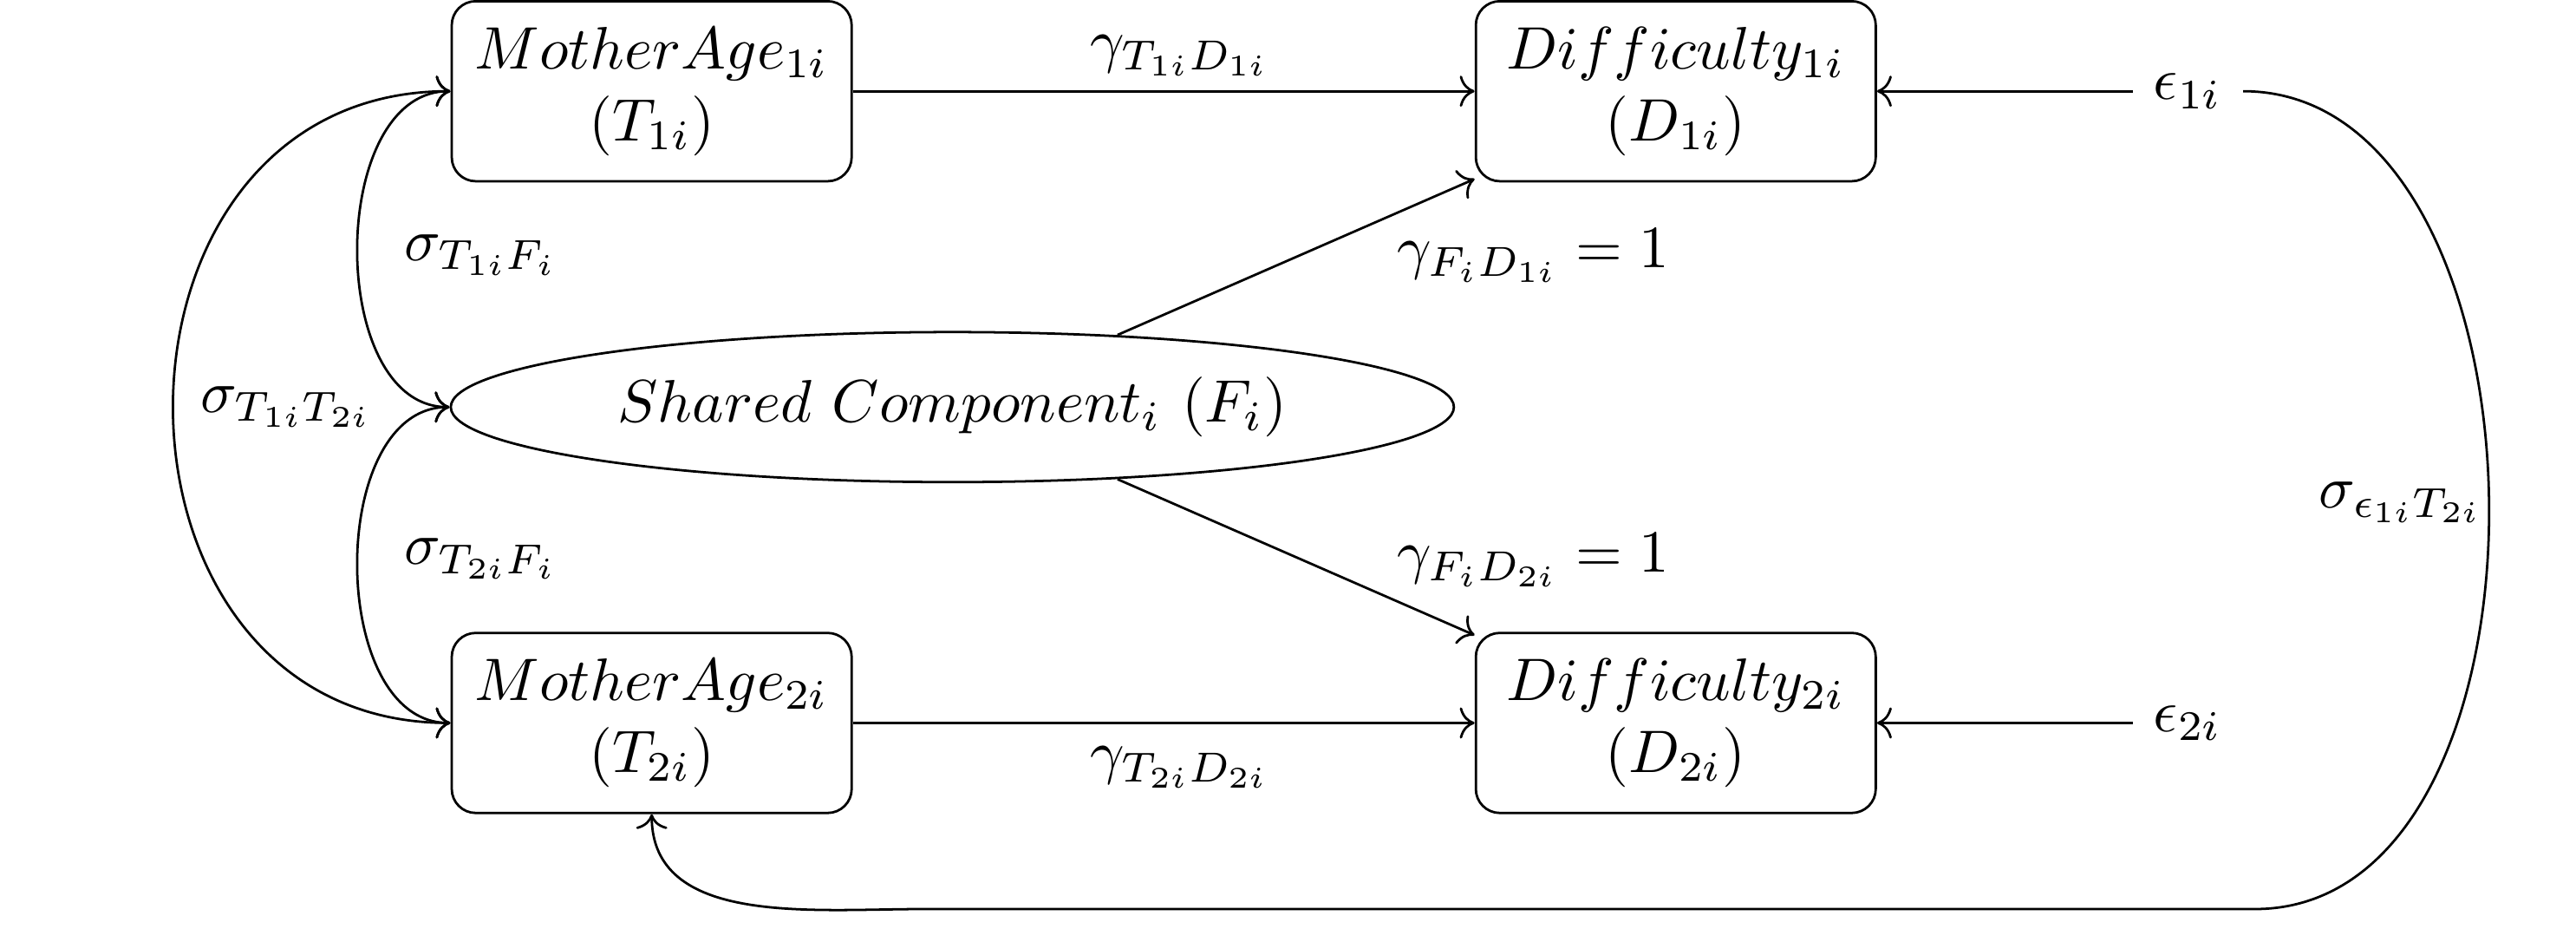
\includegraphics[width=0.8\linewidth]{diagram_model} \caption{Conceptual Model}\label{fig:diagrammodel}
\end{figure}

Figure \ref{fig:diagrammodel} depicts the conceptual model of mother's
age at birth and perceived child difficulty. T1 and T2 represent
mother's age at birth of each child which are assumed to be correlated
with one another and also with unobserved time-invariant family and
mother characteristics (or the shared component), \(FE_{i}\).
\(T_{1i}\), \(T_{2i}\), and \(FE_{i}\) predict child difficulty
(\(D_{1i}\) and \(D_{2i}\)), and the effect of the shared component is
constrained to unity for both outcomes, yielding a sibling fixed effects
model. Lastly, \(\sigma_{\epsilon_{1i},T_{2i}}\) represents the
covariance between the disturbance term for the perceived difficulty of
the first child (\(\epsilon_{1i}\)) and mother's age at second birth
(\(T_{2i}\)). Modeling this covariance accounts for the possibility that
child difficulty will impact future fertility decisions and thus timing
of future births. We hypothesize that 1) perceived difficulty of the
first child is associated with delays in subsequent births and 2) a
negative relationship between mother's age and child difficulty will
remain in the presence of any feedback effect of difficulty on second
births.

\section{Results}\label{results}

\begin{figure}
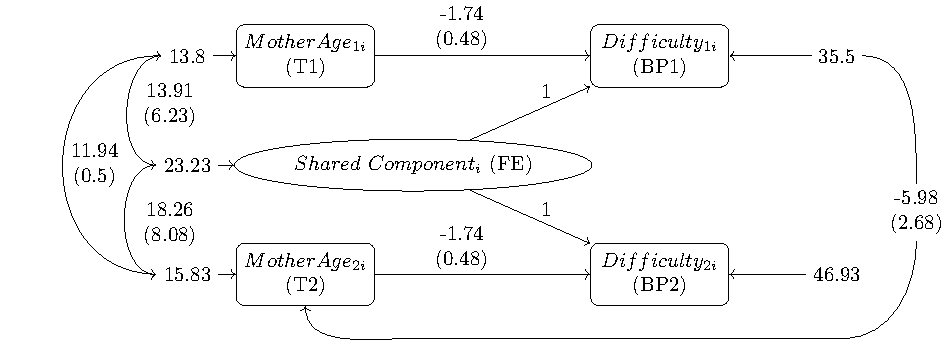
\includegraphics[width=0.8\linewidth]{diagram_estimates} \caption{Model Estimates}\label{fig:diagramestimates}
\end{figure}

Figure \ref{fig:diagramestimates} depicts maximum likelihood estimates
of the specified structural equations obtained with LISREL 9.2. A strong
negative relationship is observed between mother's age at birth of child
and perceived difficulty in early childhood. Net of time-invariant
mother and family characteristics, each additional year older at
childbirth corresponds to almost two points lower on the difficulty
composite or an approximately 1:1 relationship in standardized metrics
(B*= -0.9 and -0.94). Additionally, we see a statistically significant
(t=-2.275) relationship between the unaccounted for variation in first
child difficulty and mother's age at second birth, though this
relationship is unexpectedly negative. Greater difficulty in early
childhood, net of that associated with maternal age, appears associated
with modestly earlier second births. As the model is just identified,
tests of overall model fit cannot be conducted. For comparison the BP1
error to T2 covariance was restricted to zero to provide fit statistics,
though this restricted model is clearly misspecified given the
significance of the parameter in the full model. In this model, the root
mean square error of approximation is 0.0583 which indicates moderately
good fit, though this may be inflated by the presence of a single degree
of freedom. The restricted model chi-square is 5.731 (p=0.017),
indicating worse fit than the full (saturated) model.

\section{Discussion}\label{discussion}

These results indicate that child behavior problems may influence later
fertility decisions, rendering estimates of the effect of maternal age
biased in standard sibling models, however the effect of maternal age
remains in the presence of this feedback. This both provides support for
the findings in Hao and Matsueda (2006) regarding teen parenting and
draws attention to the importance of accounting for dynamic effects in
sibling models as described by both Rosenzweig and Wolpin (1995) and
Phillips (1999). Curiously, the feedback effect of child behavior
problems appears to be in a direction counter to expectation; positive
variation in child difficulty is associated with a shorter interval to
second birth. Extension of this analysis to include relevant covariates
from Hao and Matsueda (2006) may shed light on this finding.

While the sibling fixed effects instrumental variable model purges all
effects of unobserved time-invariant family characteristics and models
the dynamic relationship between outcomes of the first-born child and
future fertility choices, a number of key assumptions underlie the
model. First, it is assumed that there are no unaccounted for
time-variant covariates correlated with mother's age at birth and child
behavior problems. It is possible that changes in family structure and
context, particularly large shocks such as job loss or moves, influence
timing of births and child behavior problems (Phillips 1999). The
addition of time-variant family characteristics is an important next
step in this study. Second, the assumption is also made, as in Hao and
Matsueda (2006), that siblings are homogenous on relevant unobserved
characteristics; we are unable to account for unmeasured differences
between siblings related to child behavior such as differential
parenting or natural endowments. Third, it is also assumed that the
effect of mother's age at birth on child behavior problems is the same
for first and second children. A model relaxing the equivalence between
these parameters---while restricting the covariance between the
disturbance in first child's difficulty and maternal age at second
birth---yields parameter estimates that are not significantly different
(t= -1.042). Fourth, this model further assumes a linear relationship
between mother's age at birth and child behavior problems. Other
functional forms, such as a natural logarithm or quadratic term, were
tested in bivariate regressions and none offered a statistically
significant improvement in fit over a linear term, though these tests do
not rule out a more complex or subtle relationship. Lastly, our model
does not account for the possibility that difficulty of the first child
could cause mothers to cease having additional children rather than only
delaying future births. This censoring issue cannot be easily addressed
in this modeling framework and substantively lies outside the scope of
this study, however it is an important consideration which could be
addressed in future research with a hazard model relating current child
behavior to subsequent births.

\section{References}\label{references}

\hypertarget{refs}{}
\hypertarget{ref-akman_mothers_2006}{}
Akman, I. et al. 2006. ``Mothers' Postpartum Psychological Adjustment
and Infantile Colic.'' \emph{Archives of Disease in Childhood}
91(5):417--19. Retrieved March 31, 2018
(\url{http://adc.bmj.com.offcampus.lib.washington.edu/content/91/5/417}).

\hypertarget{ref-beebe_association_1993}{}
Beebe, Susan A., Rosemary Casey, and Jennifer Pinto-Martin. 1993.
``Association of Reported Infant Crying and Maternal Parenting Stress.''
\emph{Clinical Pediatrics} 32(1):15--19. Retrieved March 31, 2018
(\url{https://doi.org/10.1177/000992289303200103}).

\hypertarget{ref-bumpass_age_1978}{}
Bumpass, Larry L., Ronald R. Rindfuss, and Richard B. Jamosik. 1978.
``Age and Marital Status at First Birth and the Pace of Subsequent
Fertility.'' \emph{Demography} 15(1):75--86. Retrieved March 31, 2018
(\url{http://link.springer.com/article/10.2307/2060491}).

\hypertarget{ref-canivet_infantile_2005}{}
Canivet, Catarina A., Per-Olof Östergren, Anne-Sofie Rosén, Iréne L.
Jakobsson, and Barbro M. Hagander. 2005. ``Infantile Colic and the Role
of Trait Anxiety During Pregnancy in Relation to Psychosocial and
Socioeconomic Factors.'' \emph{Scandinavian Journal of Public Health}
33(1):26--34. Retrieved March 31, 2018
(\url{https://doi.org/10.1080/14034940410028316}).

\hypertarget{ref-carbaugh_understanding_2004}{}
Carbaugh, Suzanne Franklin. 2004. ``UNDERSTANDING SHAKEN BABY
SYNDROME:'' \emph{Advances in Neonatal Care} 4(2):105--17. Retrieved
March 31, 2018
(\url{http://content.wkhealth.com/linkback/openurl?sid=WKPTLP:landingpage\&an=00149525-200404000-00010}).

\hypertarget{ref-caspi_moving_1987}{}
Caspi, Avshalom, Glen H. Elder, and Daryl J. Bem. 1987. ``Moving Against
the World: Life-Course Patterns of Explosive Children.''
\emph{Developmental Psychology} 23(2):308--13. Retrieved March 31, 2018
(\url{http://doi.apa.org/getdoi.cfm?doi=10.1037/0012-1649.23.2.308}).

\hypertarget{ref-condeagudelo_agustin_effects_2012}{}
Conde‐Agudelo Agustín, Rosas‐Bermudez Anyeli, Castaño Fabio, and Norton
Maureen H. 2012. ``Effects of Birth Spacing on Maternal, Perinatal,
Infant, and Child Health: A Systematic Review of Causal Mechanisms.''
\emph{Studies in Family Planning} 43(2):93--114. Retrieved March 31,
2018
(\url{http://onlinelibrary.wiley.com/doi/abs/10.1111/j.1728-4465.2012.00308.x}).

\hypertarget{ref-conley_is_2000}{}
Conley, Dalton and Neil G. Bennett. 2000. ``Is Biology Destiny? Birth
Weight and Life Chances.'' \emph{American Sociological Review}
65(3):458--67. Retrieved March 31, 2018
(\url{http://www.jstor.org/stable/2657467}).

\hypertarget{ref-crowcroft_social_1997}{}
Crowcroft, N. S. and D. P. Strachan. 1997. ``The Social Origins of
Infantile Colic: Questionnaire Study Covering 76 747 Infants.''
\emph{BMJ} 314(7090):1325. Retrieved March 31, 2018
(\url{http://www.bmj.com/content/314/7090/1325}).

\hypertarget{ref-ernst_birth_2012}{}
Ernst, Cecile and Jules Angst. 2012. \emph{Birth Order: Its Influence on
Personality}. Springer Science \& Business Media.

\hypertarget{ref-furstenberg_adolescent_1987}{}
Furstenberg, Frank F., J. Brooks-Gunn, and S. Philip Morgan. 1987.
\emph{Adolescent Mothers in Later Life}. Cambridge: Cambridge University
Press. Retrieved March 31, 2018
(\url{http://ebooks.cambridge.org/ref/id/CBO9780511752810}).

\hypertarget{ref-gaysina_maternal_2013}{}
Gaysina, Darya et al. 2013. ``Maternal Smoking During Pregnancy and
Offspring Conduct Problems: Evidence from 3 Independent Genetically
Sensitive Research Designs.'' \emph{JAMA Psychiatry} 70(9):956--63.
Retrieved March 31, 2018
(\url{http://jamanetwork.com/journals/jamapsychiatry/fullarticle/1716166}).

\hypertarget{ref-geronimus_does_1994}{}
Geronimus, Arline T., Sanders Korenman, and Marianne M. Hillemeier.
1994. ``Does Young Maternal Age Adversely Affect Child Development?
Evidence from Cousin Comparisons in the United States.''
\emph{Population and Development Review} 20(3):585--609. Retrieved March
31, 2018 (\url{http://www.jstor.org/stable/2137602}).

\hypertarget{ref-griffith_childbearing_1985}{}
Griffith, Janet D., Helen P. Koo, and C. M. Suchindran. 1985.
``Childbearing and Family in Remarriage.'' \emph{Demography}
22(1):73--88. Retrieved March 31, 2018
(\url{http://link.springer.com/article/10.2307/2060987}).

\hypertarget{ref-hao_family_2006}{}
Hao, Lingxin and Ross L. Matsueda. 2006. ``Family Dynamics Through
Childhood: A Sibling Model of Behavior Problems.'' \emph{Social Science
Research} 35(2):500--524. Retrieved March 31, 2018
(\url{http://www.sciencedirect.com/science/article/pii/S0049089X04001024}).

\hypertarget{ref-kalmijn_late_2005}{}
Kalmijn, Matthijs and Gerbert Kraaykamp. 2005. ``Late or Later? A
Sibling Analysis of the Effect of Maternal Age on Children's
Schooling.'' \emph{Social Science Research} 34(3):634--50. Retrieved
March 31, 2018
(\url{http://www.sciencedirect.com/science/article/pii/S0049089X0400047X}).

\hypertarget{ref-kalmuss_subsequent_1994}{}
Kalmuss, Debra S. and Pearila Brickner Namerow. 1994. ``Subsequent
Childbearing Among Teenage Mothers: The Determinants of a Closely Spaced
Second Birth.'' \emph{Family Planning Perspectives} 26(4):149--59.
Retrieved March 31, 2018 (\url{http://www.jstor.org/stable/2136238}).

\hypertarget{ref-levine_judith_a._academic_2004}{}
Levine Judith A., Pollack Harold, and Comfort Maureen E. 2004.
``Academic and Behavioral Outcomes Among the Children of Young
Mothers.'' \emph{Journal of Marriage and Family} 63(2):355--69.
Retrieved March 31, 2018
(\url{http://onlinelibrary.wiley.com/doi/full/10.1111/j.1741-3737.2001.00355.x}).

\hypertarget{ref-mott_pace_1986}{}
Mott, Frank L. 1986. ``The Pace of Repeated Childbearing Among Young
American Mothers.'' \emph{Family Planning Perspectives} 18(1):5.
Retrieved March 31, 2018
(\url{http://www.jstor.org/stable/2135193?origin=crossref}).

\hypertarget{ref-oreopoulos_short-_2008}{}
Oreopoulos, Philip, Mark Stabile, Randy Walld, and Leslie L. Roos. 2008.
``Short-, Medium-, and Long-Term Consequences of Poor Infant Health an
Analysis Using Siblings and Twins.'' \emph{Journal of Human Resources}
43(1):88--138. Retrieved March 31, 2018
(\url{http://jhr.uwpress.org/content/43/1/88}).

\hypertarget{ref-papousek_persistent_1998}{}
Papousek, M. and N. von Hofacker. 1998. ``Persistent Crying in Early
Infancy: A Non-Trivial Condition of Risk for the Developing
Mother-Infant Relationship.'' \emph{Child: Care, Health and Development}
24(5):395--424.

\hypertarget{ref-phillips_sibship_1999}{}
Phillips, Meredith. 1999. ``Sibship Size and Academic Achievement: What
We Now Know and What We Still Need to Know: Comment on Guo and VanWey.''
\emph{American Sociological Review} 64(2):188--92. Retrieved March 31,
2018 (\url{http://www.jstor.org/stable/2657525}).

\hypertarget{ref-rao_long_2004}{}
Rao, M., R. Brenner, E. Schisterman, T. Vik, and J. Mills. 2004. ``Long
Term Cognitive Development in Children with Prolonged Crying.''
\emph{Archives of Disease in Childhood} 89(11):989--92. Retrieved March
31, 2018 (\url{https://www.ncbi.nlm.nih.gov/pmc/articles/PMC1719720/}).

\hypertarget{ref-raiha_excessively_2002}{}
Räihä, H., L. Lehtonen, V. Huhtala, K. Saleva, and H. Korvenranta. 2002.
``Excessively Crying Infant in the Family: Mother-Infant, Father-Infant
and Mother-Father Interaction.'' \emph{Child: Care, Health and
Development} 28(5):419--29.

\hypertarget{ref-rosenzweig_sisters_1995}{}
Rosenzweig, Mark R. and Kenneth I. Wolpin. 1995. ``Sisters, Siblings,
and Mothers: The Effect of Teen-Age Childbearing on Birth Outcomes in a
Dynamic Family Context.'' \emph{Econometrica} 63(2):303--26. Retrieved
March 31, 2018 (\url{http://www.jstor.org/stable/2951628}).

\hypertarget{ref-schmid_g_prospective_2010}{}
Schmid G, Schreier A, Meyer R, and Wolke D. 2010. ``A Prospective Study
on the Persistence of Infant Crying, Sleeping and Feeding Problems and
Preschool Behaviour.'' \emph{Acta Paediatrica} 99(2):286--90. Retrieved
March 31, 2018
(\url{http://onlinelibrary.wiley.com/doi/full/10.1111/j.1651-2227.2009.01572.x}).

\hypertarget{ref-sondergaard_fetal_2000}{}
Sondergaard, C., E. Skajaa, and T. B. Henriksen. 2000. ``Fetal Growth
and Infantile Colic.'' \emph{Archives of Disease in Childhood. Fetal and
Neonatal Edition} 83(1):F44--F47. Retrieved March 31, 2018
(\url{https://www.ncbi.nlm.nih.gov/pmc/articles/PMC1721113/}).

\hypertarget{ref-talvik_inga_shaken_2008}{}
Talvik Inga, Alexander Randell C, and Talvik Tiina. 2008. ``Shaken Baby
Syndrome and a Baby's Cry.'' \emph{Acta Paediatrica} 97(6):782--85.
Retrieved March 31, 2018
(\url{http://onlinelibrary.wiley.com/doi/full/10.1111/j.1651-2227.2008.00778.x}).

\hypertarget{ref-thornton_marital_1978}{}
Thornton, Arland. 1978. ``Marital Dissolution, Remarriage, and
Childbearing.'' \emph{Demography} 15(3):361--80. Retrieved March 31,
2018 (\url{http://link.springer.com/article/10.2307/2060656}).

\hypertarget{ref-wake_prevalence_2006}{}
Wake, Melissa et al. 2006. ``Prevalence, Stability, and Outcomes of
Cry-Fuss and Sleep Problems in the First 2 Years of Life: Prospective
Community-Based Study.'' \emph{Pediatrics} 117(3):836--42. Retrieved
March 31, 2018
(\url{http://pediatrics.aappublications.org/content/117/3/836}).

\subsubsection{Colophon}\label{colophon}

This report was generated on 2018-04-12 13:40:46 using the following
computational environment and dependencies:

\begin{verbatim}
#>  setting  value                       
#>  version  R version 3.4.4 (2018-03-15)
#>  system   x86_64, mingw32             
#>  ui       RTerm                       
#>  language (EN)                        
#>  collate  English_United States.1252  
#>  tz       America/Los_Angeles         
#>  date     2018-04-12                  
#> 
#>  package   * version date       source                          
#>  backports   1.1.2   2017-12-13 CRAN (R 3.4.3)                  
#>  base      * 3.4.4   2018-03-15 local                           
#>  bookdown    0.7     2018-02-18 CRAN (R 3.4.4)                  
#>  compiler    3.4.4   2018-03-15 local                           
#>  datasets  * 3.4.4   2018-03-15 local                           
#>  devtools    1.13.4  2017-11-09 CRAN (R 3.4.3)                  
#>  digest      0.6.15  2018-01-28 CRAN (R 3.4.3)                  
#>  evaluate    0.10.1  2017-06-24 CRAN (R 3.4.1)                  
#>  graphics  * 3.4.4   2018-03-15 local                           
#>  grDevices * 3.4.4   2018-03-15 local                           
#>  htmltools   0.3.6   2017-04-28 CRAN (R 3.4.1)                  
#>  knitr       1.20    2018-02-20 CRAN (R 3.4.4)                  
#>  magrittr    1.5     2014-11-22 CRAN (R 3.4.1)                  
#>  memoise     1.1.0   2017-04-21 CRAN (R 3.4.0)                  
#>  methods   * 3.4.4   2018-03-15 local                           
#>  pdftools    1.6     2018-03-27 CRAN (R 3.4.4)                  
#>  Rcpp        0.12.15 2018-01-20 CRAN (R 3.4.3)                  
#>  rmarkdown   1.9     2018-03-01 CRAN (R 3.4.4)                  
#>  rprojroot   1.3-2   2018-01-03 CRAN (R 3.4.3)                  
#>  stats     * 3.4.4   2018-03-15 local                           
#>  stringi     1.1.6   2017-11-17 CRAN (R 3.4.2)                  
#>  stringr     1.3.0   2018-02-19 CRAN (R 3.4.4)                  
#>  tools       3.4.4   2018-03-15 local                           
#>  utils     * 3.4.4   2018-03-15 local                           
#>  withr       2.1.2   2018-04-04 Github (jimhester/withr@79d7b0d)
#>  xfun        0.1     2018-01-22 CRAN (R 3.4.4)                  
#>  yaml        2.1.16  2017-12-12 CRAN (R 3.4.3)
\end{verbatim}


\end{document}
